% --------------------- VARIABLEN -------------------------

\newcommand{\COURSE}{Physik und Materialwissenschaften\\ Praktikum Physik \\}
\newcommand{\SEMESTER}{Elektro- und Informationstechnik II}
\newcommand{\STUDENT}{Maximilian Spahn\\ und\\Benjamin Langer}

\newcommand{\HEADDING}{Praktikum Physik}
\newcommand{\SUBHEADDING}{Versuch 4.3: Wärmestrahlung und Konvektion}

% ------------------- DEFINITIONEN -----------------------

\documentclass[a4paper]{scrartcl}

\usepackage[utf8]{inputenc}
\usepackage[ngerman]{babel}
\usepackage{amsmath}
\usepackage{amssymb}
\usepackage{color}
\usepackage{tikz}
\usepackage{float}
\usetikzlibrary{arrows,decorations.markings}
\usepackage{tabularx}
\usepackage{fancybox}
\usepackage{pgfplots}
\usepackage[colorlinks=false,linkcolor=black,urlcolor=blue,bookmarks,bookmarksopen=true]{hyperref}
\usepackage{geometry}
\usepackage{fancyhdr}
\usepackage{subcaption}

\usepackage[page]{totalcount}

%Größe der Ränder setzen
\geometry{a4paper,left=2cm, right=2cm, top=3cm, bottom=2cm, headheight=8cm}

%Kopf- und Fußzeile
\pagestyle {fancy}
\fancyhf{}
\fancyhead[L]{\STUDENT}
\fancyhead[C]{\COURSE}
\fancyhead[R]{\today}

\fancyfoot[L]{\SEMESTER}
\fancyfoot[C]{}
\fancyfoot[R]{Seite \thepage /\pageref{LastPage}}

%Formatierung der Überschrift, hier nichts ändern
\def\header#1#2{
  \begin{center}
    {\Large #1}\\
    {#2}
  \end{center}
}

\numberwithin{equation}{subsection} 

\nocite{*}
\bibliographystyle{plainurl}

\setlength\parindent{0pt}

% ----------------------- DOCUMENT ---------------------------

\begin{document}

\vspace{10pt}
\header{\HEADDING}{\SUBHEADDING}

\tableofcontents

\newpage

\section{Einleitung}
\subsection{Wärmestrahlung}

Beim ersten Versuchsteil geht es darum mit Hilfe einer Infrarot-Kamera Wärmestrahlung zu beobachten.
Zuerst wird eine Glühbirne verwendet und später ein Infrarotstrahler.
An der Glühbirne wird zusätzlich mit Hilfe eines Pyrometers die Temperatur gemessen.

\subsection{Konvektion}
Bei diesem Versuchsteil soll gezeigt werden, dass verschiedene Temperaturen bei verschiedenen Dichten zu Auftriebskräften führt.
Dieser Versuchsteil ist größtenteils mit Bildern dokumentiert.\\
Im folgenden werden die Ergebnisse der Versuche dargestellt.

\newpage
\section{Theorie}
\subsection{Teil A: Wärmestrahlung}
Licht ist eine Elektromagnetische Welle.
Wir Menschen können allerdings nur ein sehr kleines Spektrum davon sehen (zwischen $\lambda = 400\;nm$ und $\lambda = 750\;nm$).
Strahlung, die eine größere Wellenlänge hat wird Infrarotstrahlung genannt.
Dabei unterscheidet man:

\begin{align*}
&\textbf{Nahe Infrarotstrahlung:}&800\;nm &< \lambda < 3\;\mu m\\
&\textbf{Mittlere Infrarotstrahlung:}&3\;\mu m &< \lambda < 6\;\mu m\\
&\textbf{Ferne Infrarotstrahlung:}&6\;\mu m &< \lambda < 1\;mm
\end{align*}

Infrarotstrahlung kann entstehen, wenn ein Elektron von einem energetisch höheren Zustand in einen niedrigeren wechselt.
Die Energiedifferenz wird in Form von IR-Strahlung abgegeben.
Dabei hängt die Energiedifferenz $\Delta E$ mit der Frequenz $f$ und der Wellenlänge $\lambda$ wie folgt zusammen:

\begin{align}
\Delta E = h \cdot f = h \cdot \frac{c}{\lambda}
\end{align}

Ebenso kann IR-Strahlung auch von heißen Festkörpern emittiert werden.
Das liegt daran, dass der Festkörper durch die Erwärmung anfängt zu schwingen und elektrische Ladungen beschleunigt werden.
Dies führt zur Emission von Strahlung.
Man spricht von einem Temperaturstrahler.

\subsubsection{Wiensches Verschiebungsgesetz}

\begin{figure}[H]
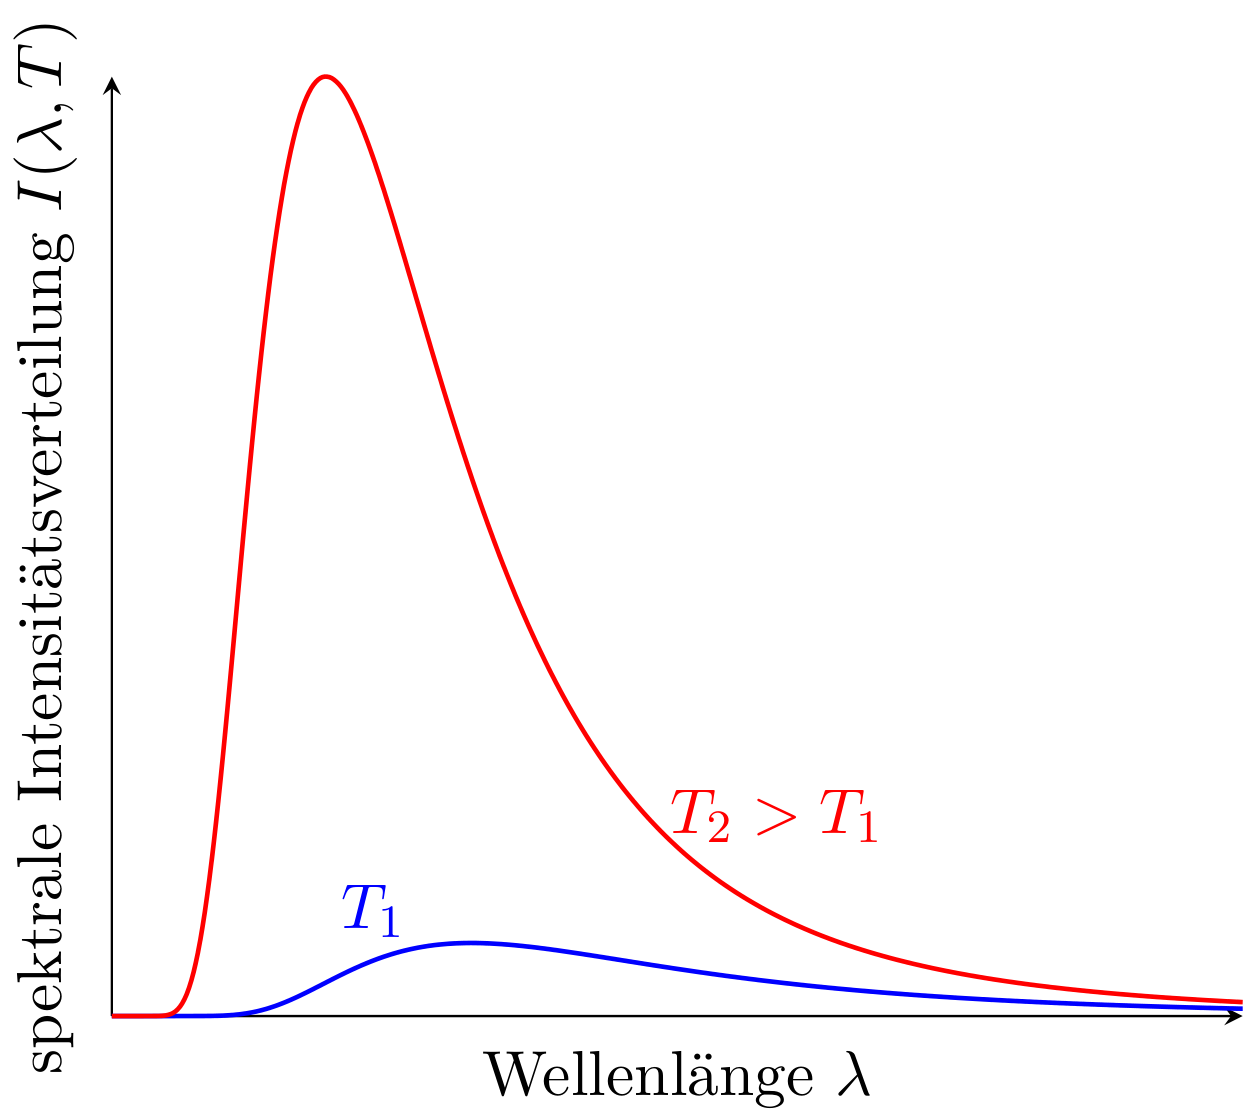
\includegraphics[width=10cm]{Abbildungen/Wien}
\centering
\caption{Spektrale Intensitätsverteilung eines Temperaturstrahlers \cite{anl}}
\centering
\label{fig:wien}
\end{figure}

In Abbildung \ref{fig:wien} ist die Intensitätsverteilung eines Temperaturstrahlers in Abhängigkeit von der Wellenlänge aufgetragen.
Man sieht, dass mit zunehmender Temperatur das Maximum der Intensität bei immer kleineren Wellenlängen ist.
Das ist die sich ändernde Farbe beim aufheizen von Metall.
Die Lage des Maximums lässt sich mit dem Wienschen Verschiebungsgesetz berechnen:

\begin{align}
\label{eq:wien}
\lambda_{max} = \frac{b}{T}
\end{align}

mit WIEN-Konstante:

\begin{align*}
b = 2,9 \times 10^{-3}\;m \cdot K
\end{align*}

\subsubsection{Stefan-Boltzmann-Gesetz}
In Abbildung \ref{fig:wien} lässt sich außerdem erkennen, dass sich die Gesamtintensität aller abgestrahlten Wellenlänge (Fläche unter der Kurve) mit zunehmender Temperatur vergrößert.
Diese Gesamtintensität kann man mit dem Stefan-Boltzmann-Gesetz berechnen:

\begin{align}
\label{eq:StBo}
I_{ges} \sim \sigma \cdot T^4
\end{align}

mit Stefan-Boltzmann-Konstante:

\begin{align*}
\sigma = 5,67 \times 10^{-8}\; \frac{W}{m^2 K^4}
\end{align*}

\subsubsection{Strahlungsgesetz von Planck}
Die in Abbildung \ref{fig:wien} dargestellte Kurve konnte zuerst um 1900 von Max Planck analytisch beschrieben werden.
Sie wird durch das Strahlungsgesetz von Planck beschrieben:

\begin{align}
\label{eq:Planck}
M(\lambda,T)=\frac{2\cdot\pi\cdot h\cdot c^2}{\lambda^5}\frac{1}{e^{\frac{h\cdot c}{k\lambda T}}-1}
\end{align}

Die Formel beschreibt, dass Strahlung in Form von Photonen nur gequantelt auftritt.
Die beiden Gesetze von Wien \ref{eq:wien} und Stefan-Boltzmann \ref{eq:StBo} können jederzeit aus der Gleichung \ref{eq:Planck} hergeleitet werden.

\subsubsection{Kirchhoff-Gesetz}
Ein Körper, der die gesamte auftreffende Strahlung absorbieren kann wird \glqq schwarzer Körper\grqq genannt.
Die bisher genannten Gleichungen beziehen sich auf schwarze Körper.
In der Realität kommen aber nur Körper vor, welche nur einen Teil der Strahlung absorbieren.
Diese nennt man \glqq graue Körper\grqq.\\
Der Absorptionsgrad $\alpha$ ist das Verhältnis zwischen absorbierter Strahlung und auftreffender Strahlung.\\
Für schwarze Körper liegt $\alpha$ bei 1, für einen Spiegel (\glqq weißer Körper\grqq) bei 0 und für graue Körper zwischen 0 und 1.\\
Für den Emissionsgrad $\varepsilon$ kann man einen ähnlichen Zusammenhang definieren.\\
Laut dem Kirchhoff-Strahlungsgesetz ist bei einer bestimmten Temperatur $T$ und Wellenlänge $\lambda$ der Emissionsgrad $\varepsilon$ gleich dem Absorptionsgrad $\alpha$:

\begin{align*}
\varepsilon(T,\lambda)=\alpha(T,\lambda)
\end{align*}

Man kann dies benutzen um \glqq Kantenfilter\grqq zu bauen, die wie ein Hochpass für Wellenlängen wirken.
Unterhalb einer bestimmten Grenzwellenlängen, wir die gesamte Strahlung absorbiert, darüber durchgelassen.

\subsection{Teil B: Infrarotbildtechnik}
\subsubsection{Grenzwellenlänge}
Ein Halbleiter kann ein Photon nur absorbieren, wenn die Energie des Photons größer als die Energie der Bandlücke ist.
Die maximale Wellenlänge der Strahlung die absorbiert werden kann nennt man Grenzwellenlänge $\lambda_G$.

\begin{align}
\label{eq:grenz}
\lambda_G < \frac{h\cdot c}{E_{Gap}}
\end{align}

\subsubsection{IR-Reflexion}
Infrarotstrahlen werden auch z.B. in der Sicherheitstechnik verwendet.
Dabei werden Infrarotstrahlen mit einem Infrarotstrahler entsandt und die reflektierten Infrarotstrahlen detektiert.

\subsection{Teil C: Konvektion}
Bei einer Temperaturdifferenz zwischen verschiedenen Schichten von einer Flüssigkeit oder eines Gases gibt es Auftriebskräfte.
Die heißeren, weniger dichten Flüssigkeiten oder Gase treiben im Vergleich zu den kalten nach oben.
Dieser Effekt wird unter anderem bei Kühlkörpern verwendet.

\newpage
\section{Häusliche Vorarbeit}
\subsection{Teil A: Wärmestrahlung}
\subsubsection{Beschreibung der Auslegung eines Kühlkörpers für optimale Wärmestrahlung}
Auf der Abbildung \ref{fig:kuehl} sieht man zwei verschiedene Möglichkeiten für die Rippenanordnung eines Kühlkörpers.
Dabei ist die linke Variante besser als die rechte.
Das liegt daran, dass durch die sternförmige Anordnung die Wärmestrahlung besser emittiert werden kann.
Bei der Variante auf der rechten Seite, wird die Wärmestrahlung zwar auch emittiert, aber durch die parallele Anordnung der Kühlrippen wird ein Großteil der Strahlung wieder absorbiert.
Dadurch kühlt die rechte Anordnung schlechter ab.

\begin{figure}[H]
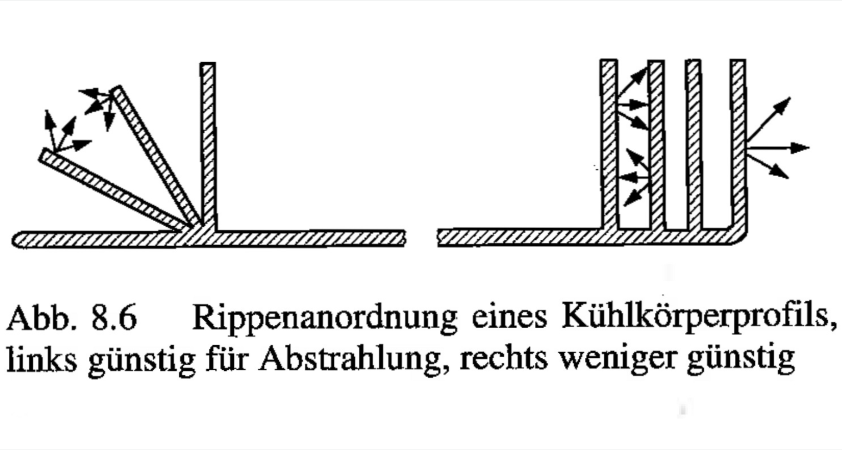
\includegraphics[width=12cm]{Abbildungen/Kuehlkoerper}
\centering
\caption{Beispiel von Leute für die Rippenanordnung von Kühlkörpern \cite{anl}}
\centering
\label{fig:kuehl}
\end{figure}

\subsubsection{Berechnen der IR-Photonen}
Die Anzahl der IR-Photonen pro Sekunde werden mit der folgenden Formel berechnet:

\begin{align*}
N = \frac{I}{E} = \frac{I\cdot \lambda}{h\cdot c} = 20\;\frac{mW}{cm^2} \cdot 1\;\mu m \cdot 5,03\times 
10^{24} = 100,68\times 10^{15}
\end{align*}

\subsubsection{Nehmen Sie an, Ihr Schornsteinfeger sei ein schwarzer Strahler}
Wenn man annimmt, dass ein Schornsteinfeger ein schwarzer Strahler sei, lässt sich seine Strahlungsintensität nach dem Stefan-Boltzmann-Gesetz berechnen (\ref{eq:StBo}).
Dabei nimmt man für die Temperatur eine Körpertemperatur von $310,15\;K$ an.

\begin{align*}
I_{ges}\sim\sigma\cdot (310,15\;K)^4 \approx 524,68\;\frac{W}{m^2}
\end{align*}

Die Wellenlänge seiner maximalen Strahlungsintensität lässt sich mit dem Wienschen Verschiebungsgesetz berechnen (\ref{eq:wien}).

\begin{align*}
\lambda_{max} = \frac{b}{310,15\;K} = 9,35\; \mu m
\end{align*}

\subsection{Teil B: Infrarotbildtechnik}
\subsubsection{Bandlücken und Grenzwellenlängen für Si, Ge, GaAs}
Die Grenzwellenlängen für die verschiedenen Halbleiter lassen sich mit der Formel \ref{eq:grenz} berechnen.\\
Si ($1,11\;eV$):

\begin{align*}
\lambda_{G_{Si}} < \frac{h \cdot c}{1,11\cdot 1,602\times 10^{-19}\;J} = 1100\;nm 
\end{align*}
Ge ($0,66\;eV$):

\begin{align*}
\lambda_{G_{Ge}} < \frac{h \cdot c}{0,66\cdot 1,602\times 10^{-19}\;J} = 1850\;nm 
\end{align*}
GaAs ($1,43\;eV$):
\begin{align*}
\lambda_{G_{GaAs}} < \frac{h \cdot c}{1,43\cdot 1,602\times 10^{-19}\;J} = 850\;nm 
\end{align*}

\newpage
\section{Aufbau und Durchführung}
\subsection{Teil A: Wärmestrahlung}
Der Versuchsaufbau ist in Abbildung \ref{fig:AufbauA} dargestellt.

\begin{figure}[H]
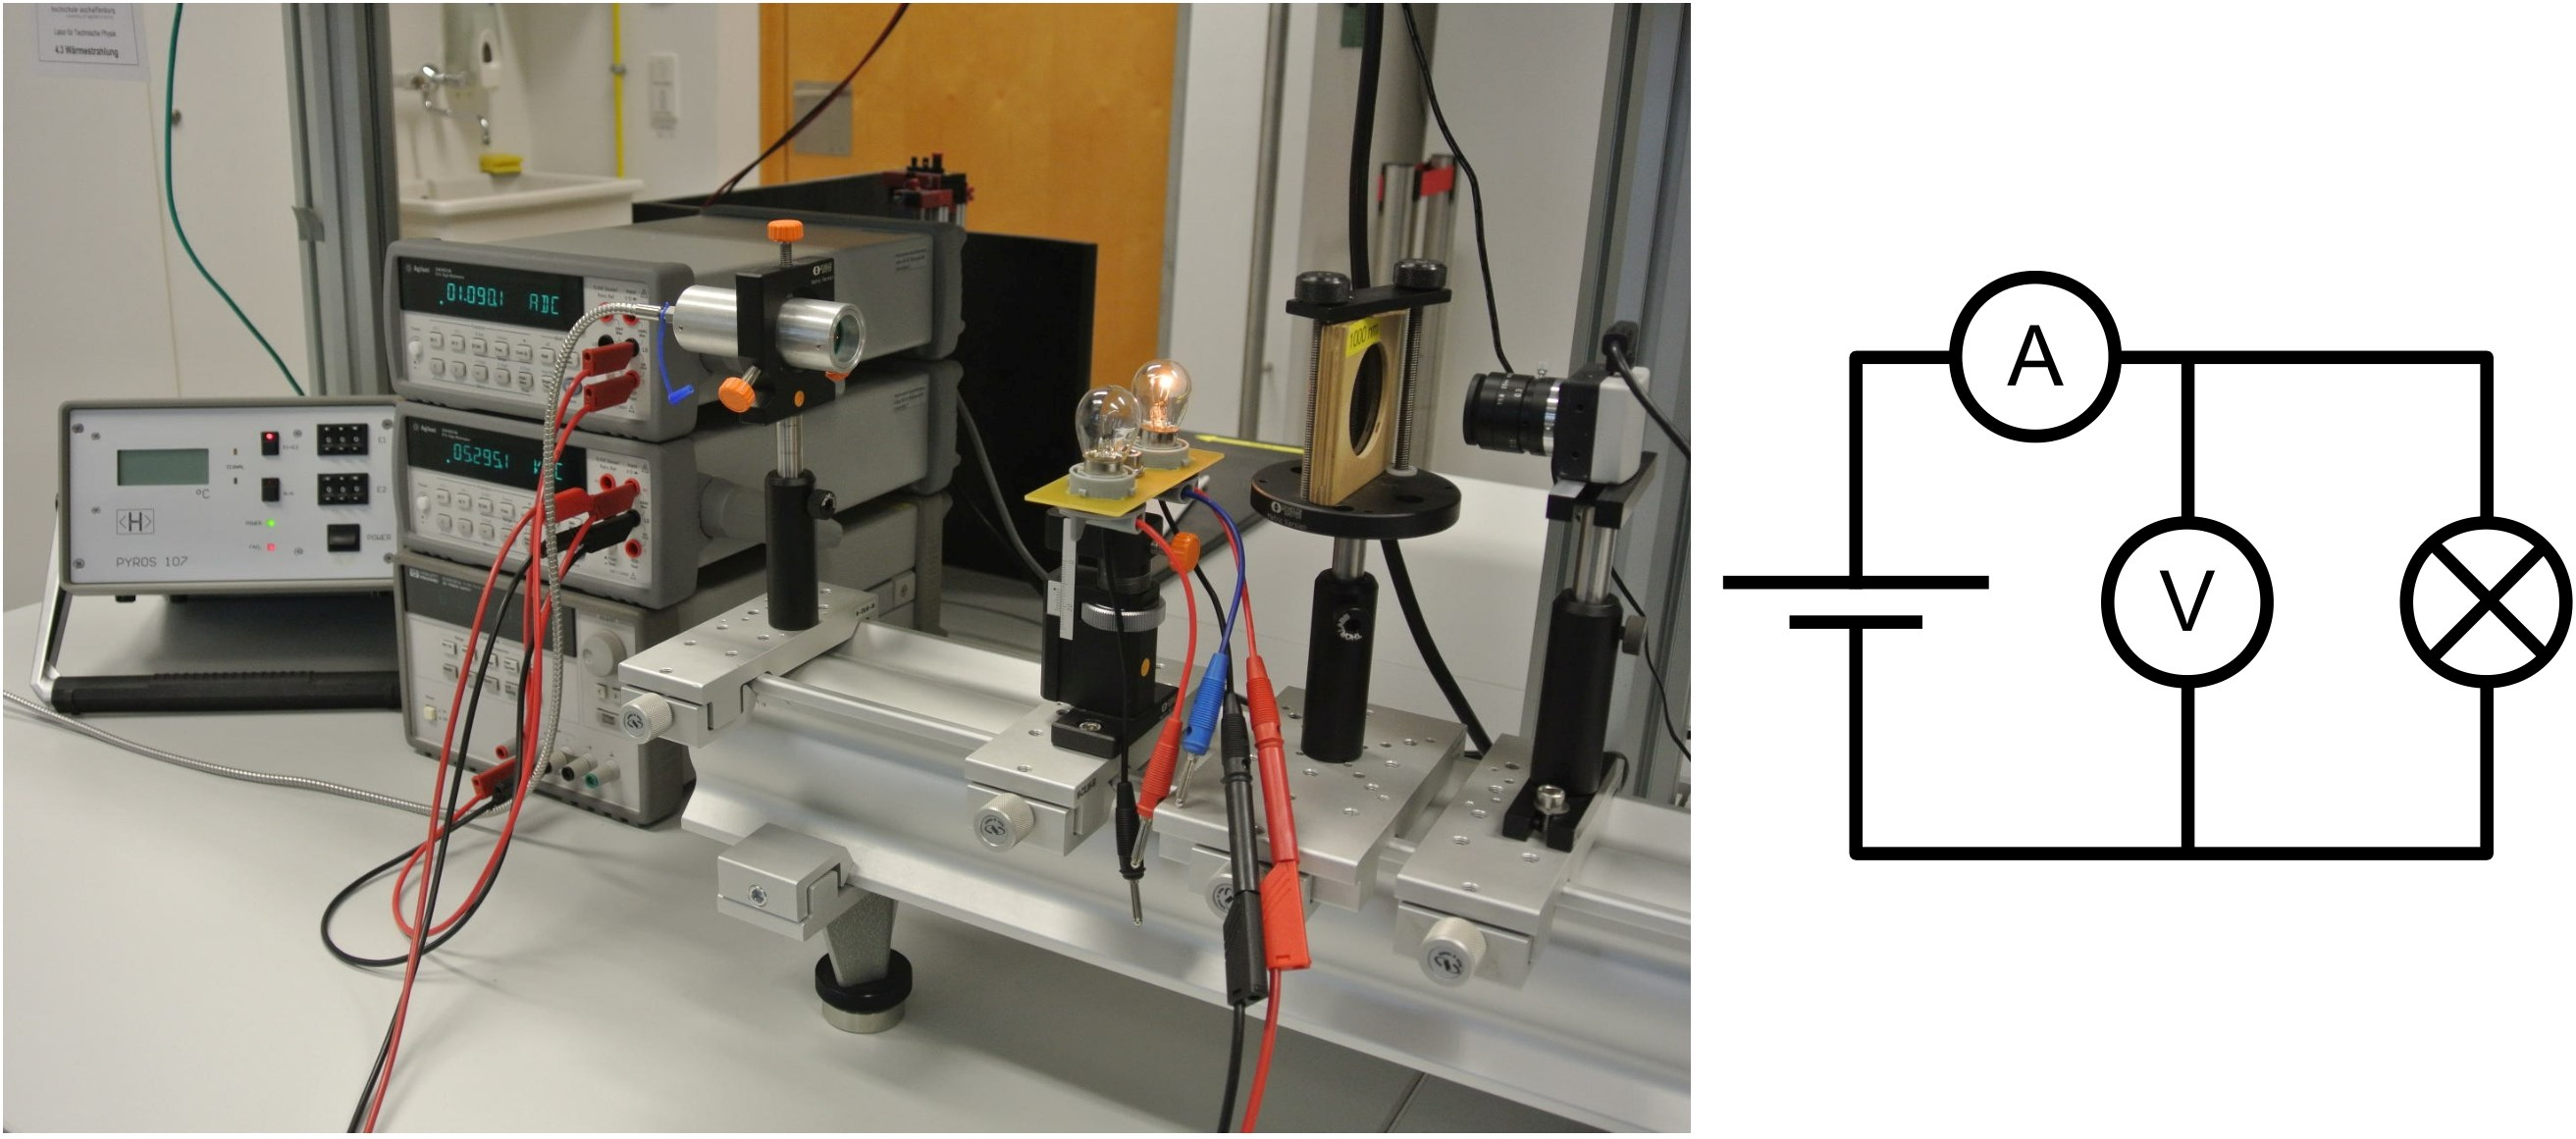
\includegraphics[width=12cm]{Abbildungen/AufbauA}
\centering
\caption{Versuchsaufbau für Teil A \cite{anl}}
\centering
\label{fig:AufbauA}
\end{figure}

Mit dem Heizstrom der Glühbirne lässt sich die Temperatur der Glühwendel verändern.
Die Temperatur wird kontaktlos mit Hilfe eines Pytometers gemessen.

\subsection{Teil B: Infrarotbildtechnik}
Der Versuchsaufbau ist in Abbildung \ref{fig:AufbauB} dargestellt.

\begin{figure}[H]
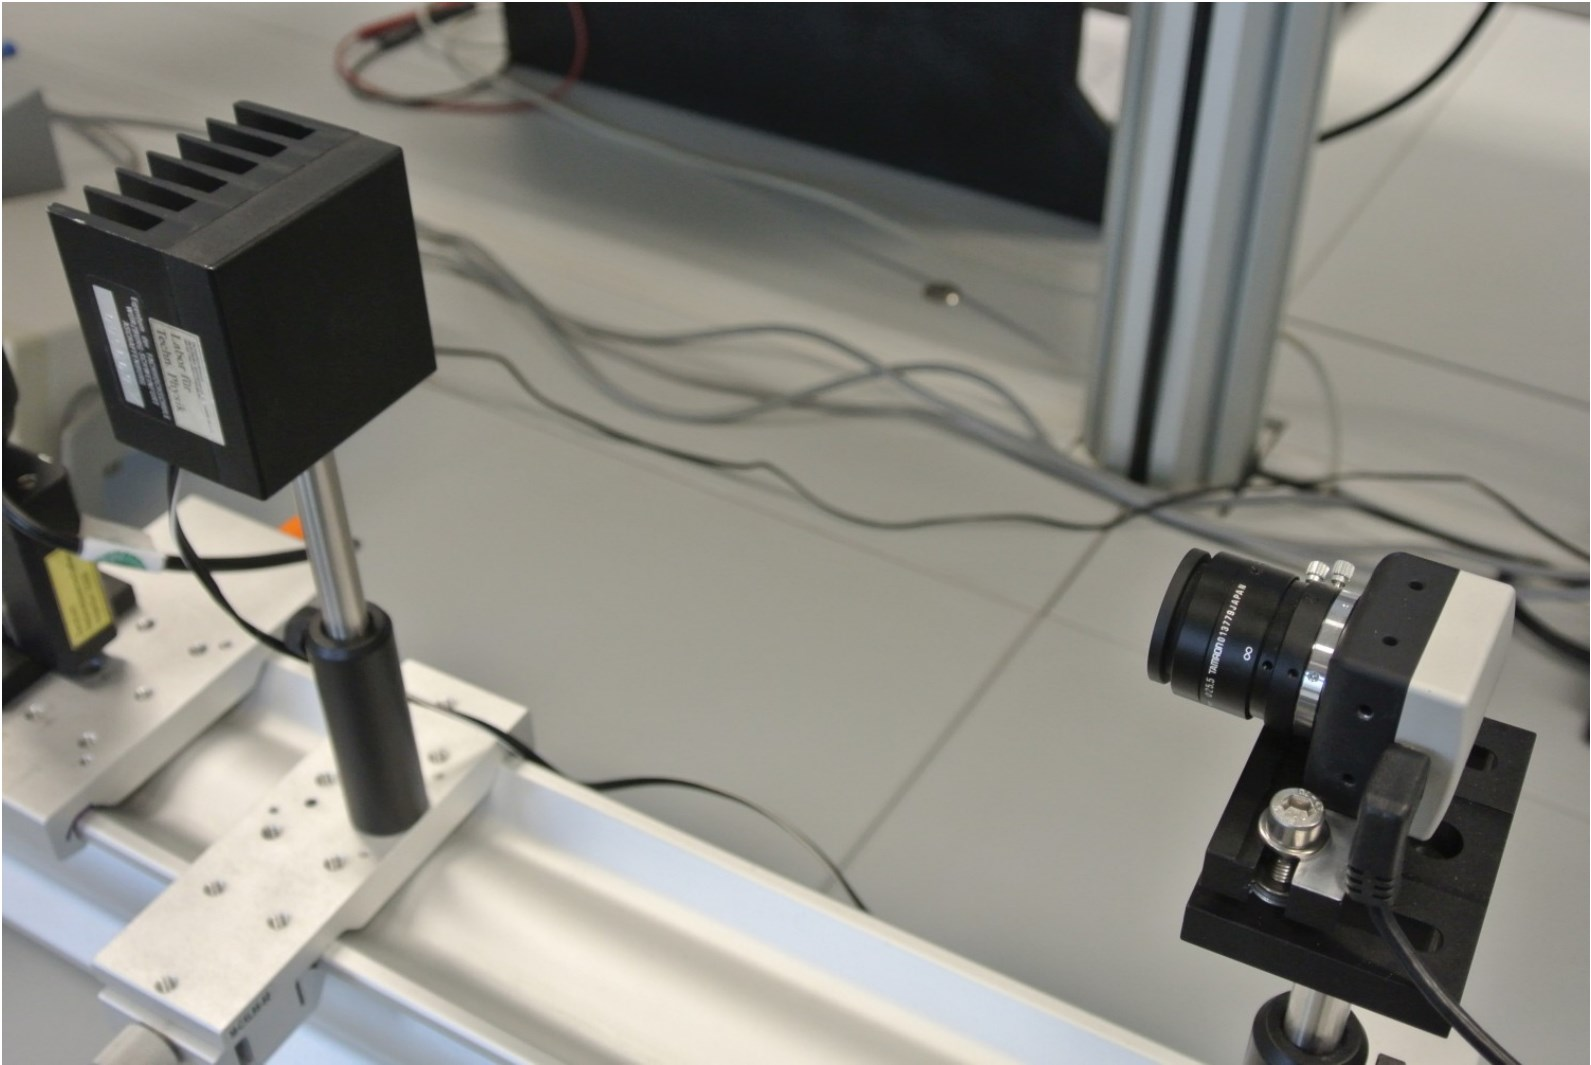
\includegraphics[width=11cm]{Abbildungen/AufbauB}
\centering
\caption{Versuchsaufbau für Teil A \cite{anl}}
\centering
\label{fig:AufbauB}
\end{figure}
\subsection{Teil C: Konvektion}
Der Versuchsaufbau ist in Abbildung \ref{fig:AufbauC} dargestellt.

\begin{figure}[H]
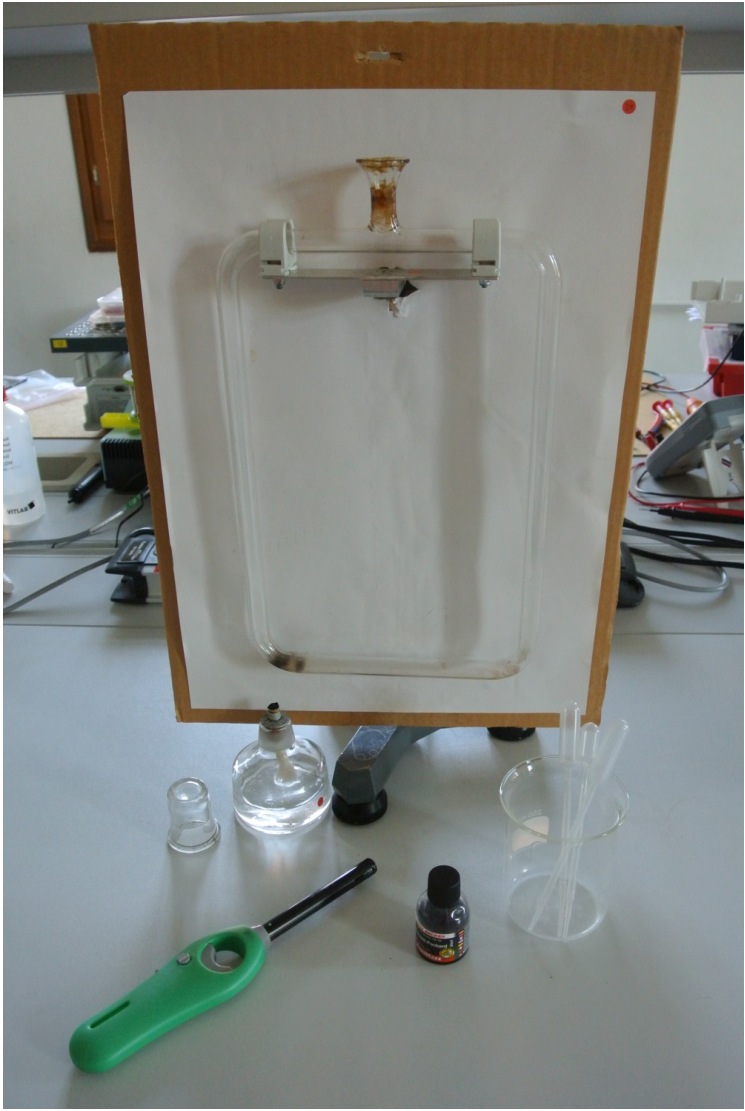
\includegraphics[width=10cm]{Abbildungen/AufbauC}
\centering
\caption{Versuchsaufbau für Teil A \cite{anl}}
\centering
\label{fig:AufbauC}
\end{figure}

In ein Konvektionsrohr wird Wasser gefüllt, bis sich ein geschlossener Wasserkreislauf bildet.
An der unteren Seite wird ein Spiritusbrenner positioniert.
In die Öffnung wird Druckertinte gegeben, wodurch man Konvektion beobachten kann.

\newpage
\section{Auswertung Versuch}
\subsection{Teil A: Wärmestrahlung}
Kaltwiderstand Glühfaden $R_0$ bei Raumtemperatur $T_0$:

\begin{align*}
R_0 &= (0,86\pm 0,15)\;\Omega\\
T_0 &= (23\pm 1)\;^\circ C
\end{align*}

Die Spannung und der Strom des Glühfadens wurden in 100$^\circ C$  Schritten von 900$^\circ C$ bis 2500$^\circ C$ gemessen.
Daraus wird der Widerstand des Glühfadens berechnet.
Die Messwerte sind im Anhang beigefügt (Abschnitt \ref{sec:Anhang}/ Tabelle \ref{tab:Messwerte}).\\
Mit dem $1\;\mu m$-Kantenfilter vor dem Objektiv der Kamera werden nur noch Wellen im Wellenlängenbereich $>1\;\mu m$ angezeigt.\\
Danach wird der Widerstand des Glühfadens gemessen, wenn er einmal mit und einmal ohne Kamera gerade so zu glühen beginnt.
Da zunächst Strom und Spannung gemessen wurden, muss der Widerstand mit Fehlerfortpflanzung berechnet werden:

\begin{align*}
R = \frac{U}{I}
\end{align*}

\begin{align*}
&\frac{\partial R}{\partial U} = \frac{1}{I}
&\frac{\partial R}{\partial I} = - \frac{U}{I^2}
\end{align*}

\begin{align}
U_R = \bigg | \frac{\partial R}{\partial U} \bigg | \cdot U_U + \bigg | \frac{\partial R}{\partial I} \bigg | \cdot U_I
\end{align}

mit Kamera:
\begin{align*}
R&=(1,84\pm 0,12)\;\Omega\\
T&=(541 \pm 1)\;^\circ C
\end{align*}

mit bloßem Auge:
\begin{align*}
R&=(2,25\pm 0,12)\;\Omega\\
T&=(768 \pm 1)\;^\circ C
\end{align*}

Die Widerstände wurden in Abhängigkeit von der Temperatur graphisch dargestellt (sieh Abschnitt \ref{sec:Anhang}/ Abbildung \ref{fig:Diagramm}).

\subsection{Teil B: Infrarotbildtechnik}
Bei dem vorhanden Infrarot-Strahler handelt es sich um einen Diodenstrahler (sieh Abbildung \ref{fig:IR}).
Man konnte keine Funktionsfehler erkennen.
Nur auf der Abdeckung konnte man erkennen, wo diese gegossen wurde.
\subsection{Teil C: Konvektion}

\begin{figure}[H]
\begin{subfigure}{4cm}
\centering
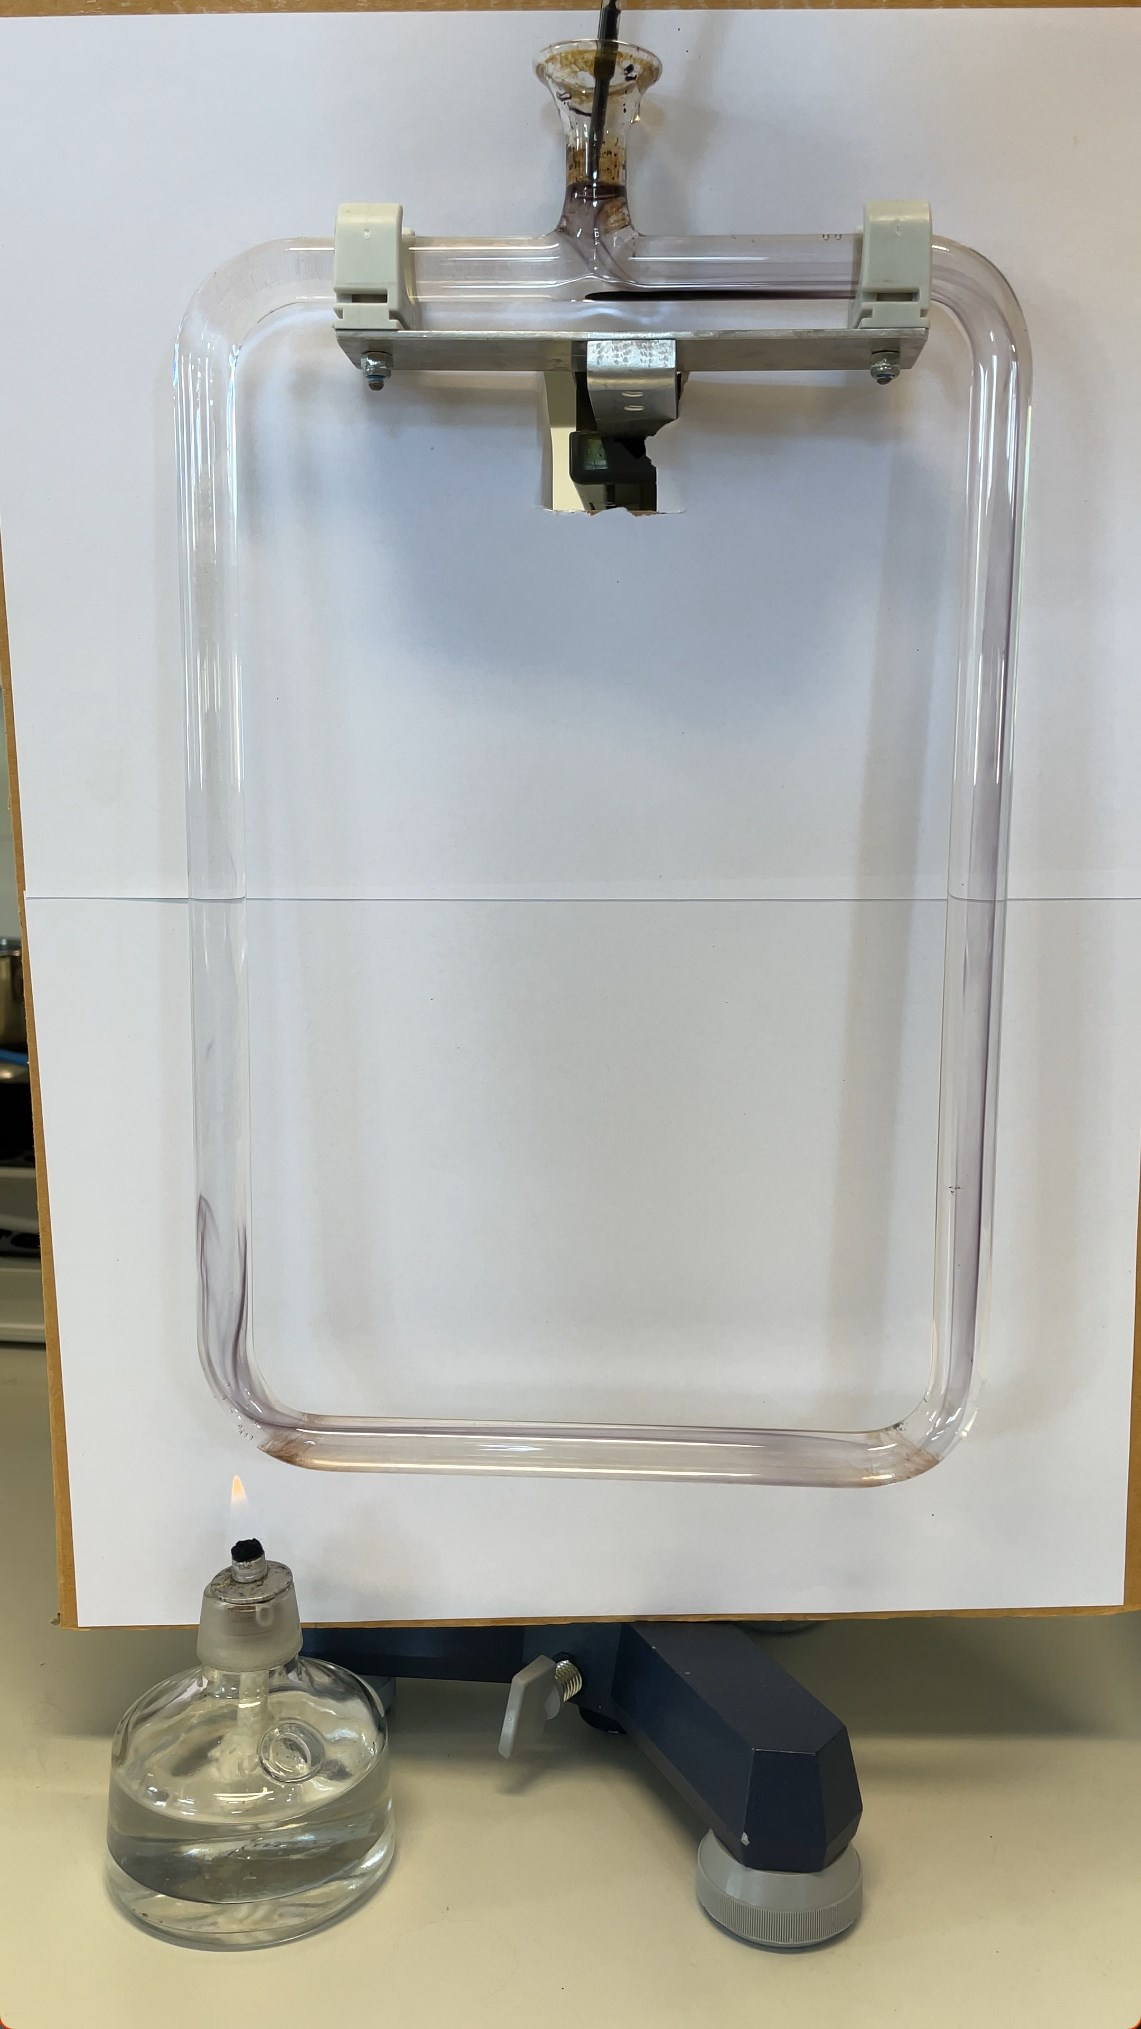
\includegraphics[width=4cm]{Abbildungen/1}
\caption{}
\label{a}
\end{subfigure}
\begin{subfigure}{4cm}
\centering
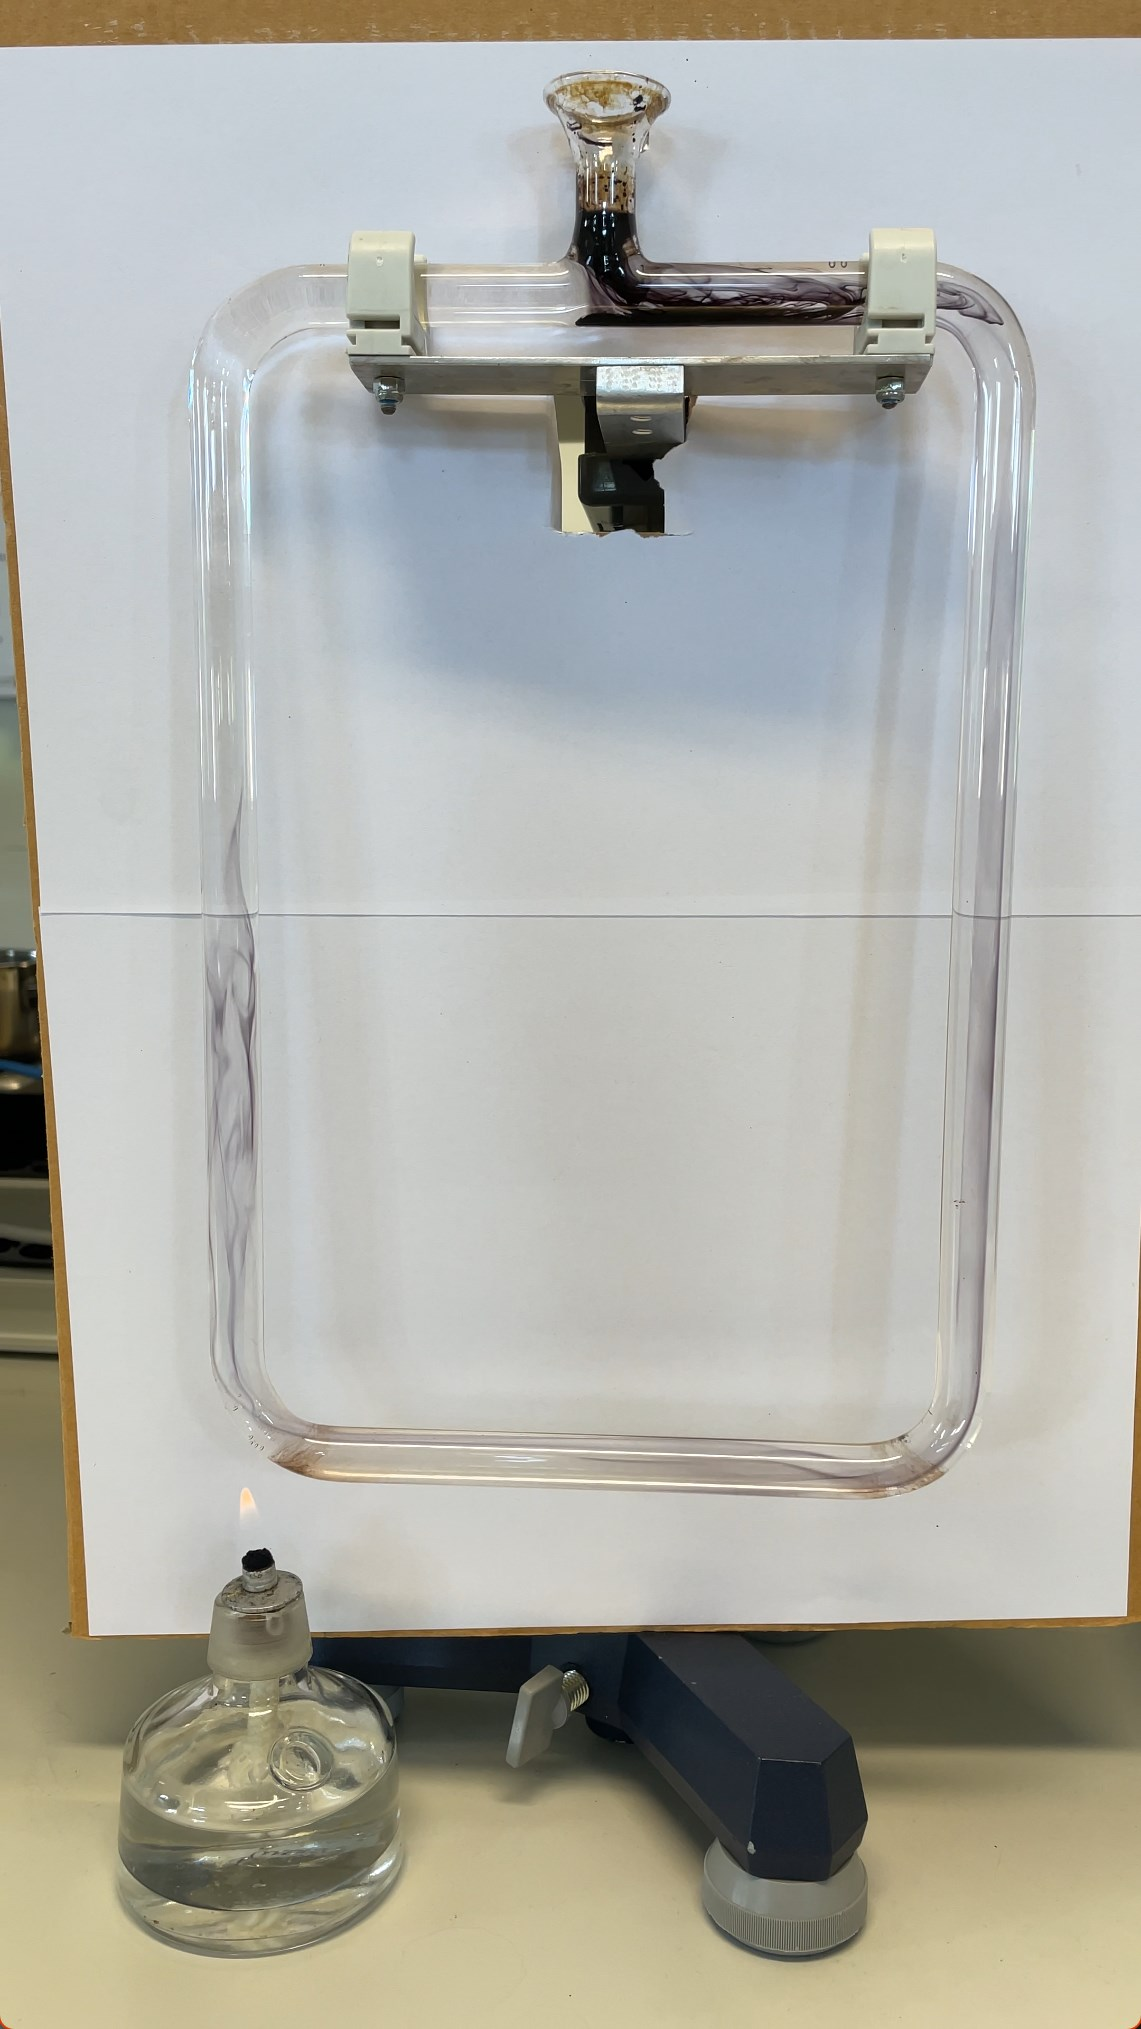
\includegraphics[width=4cm]{Abbildungen/2}
\caption{}
\label{b}
\end{subfigure}
\begin{subfigure}{4cm}
\centering
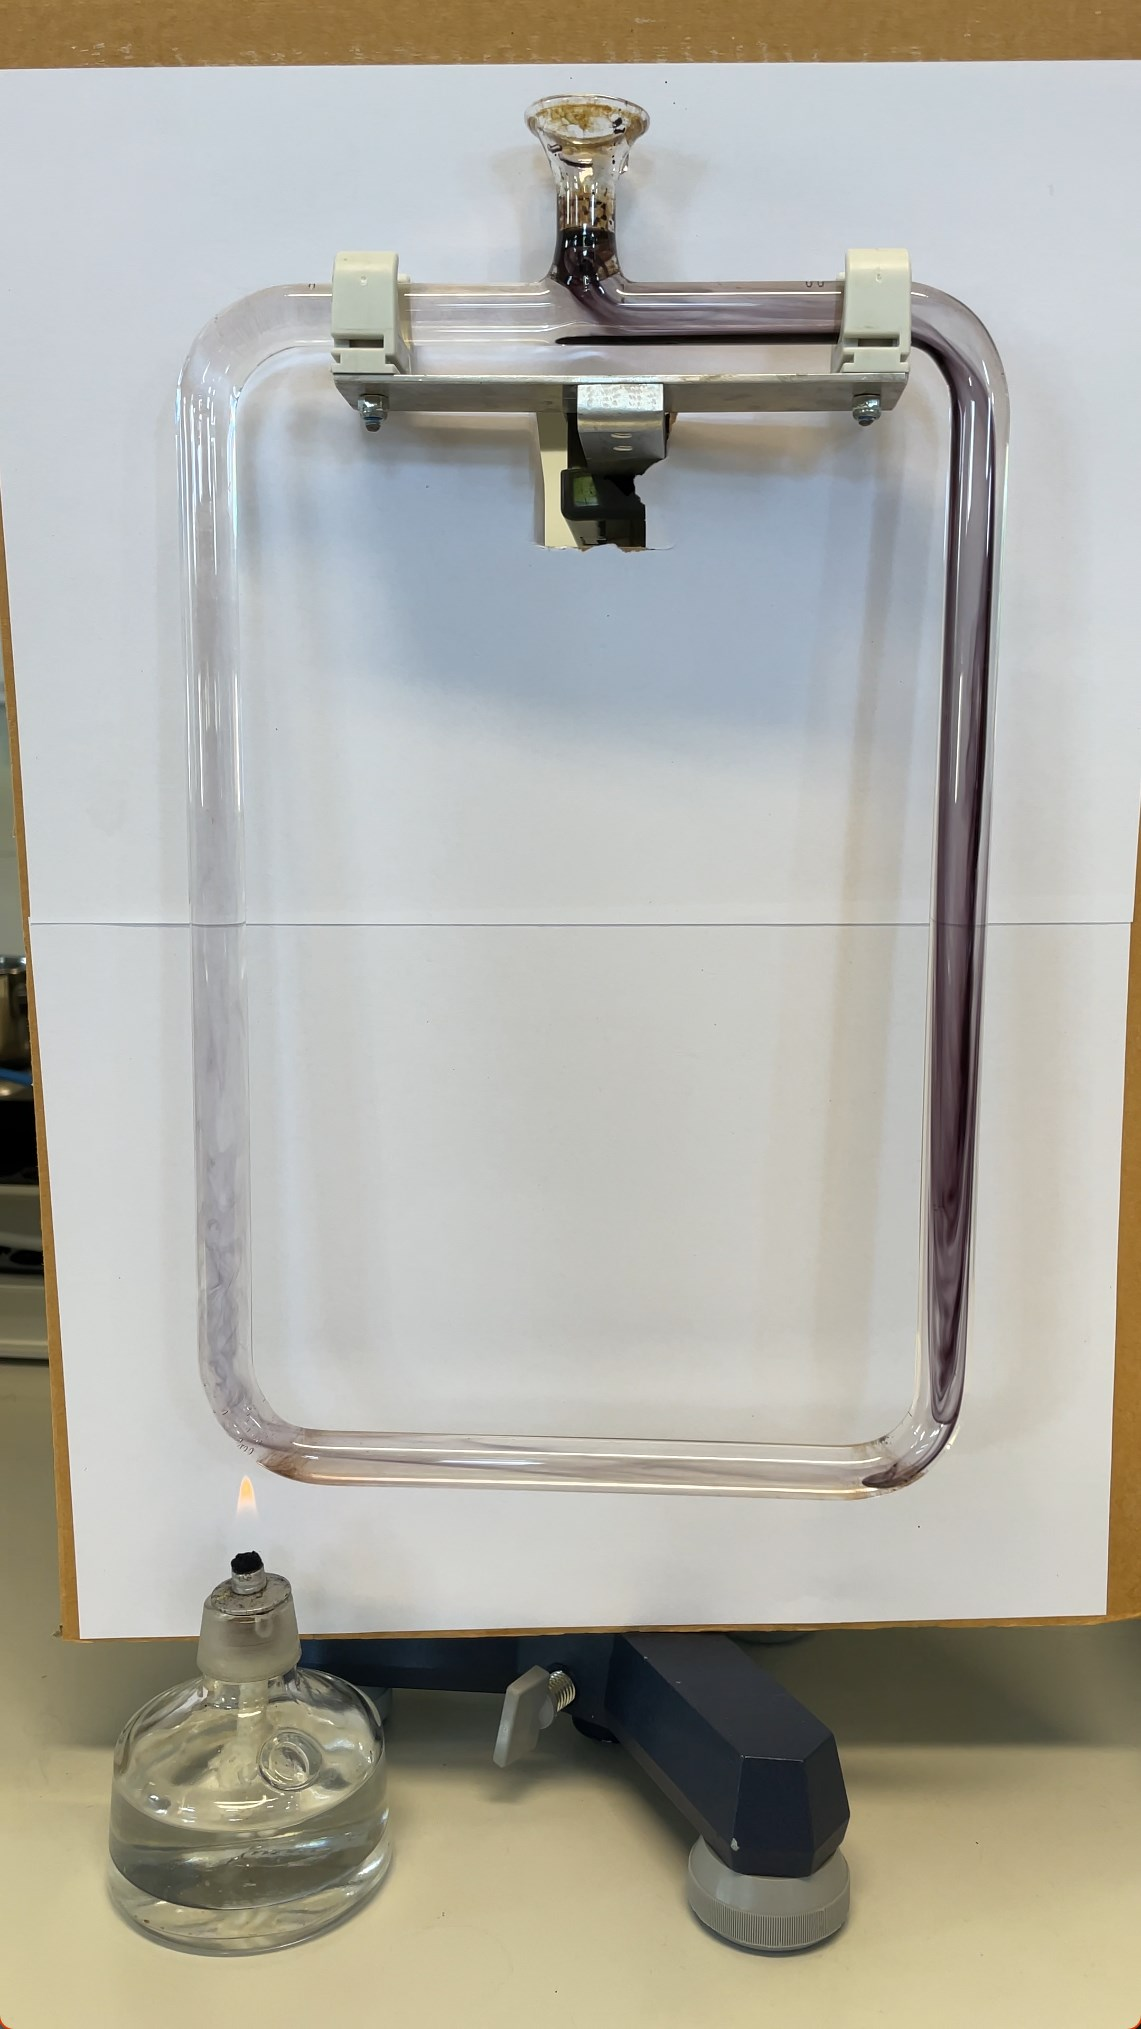
\includegraphics[width=4cm]{Abbildungen/3}
\caption{}
\label{c}
\end{subfigure}
\begin{subfigure}{4cm}
\centering
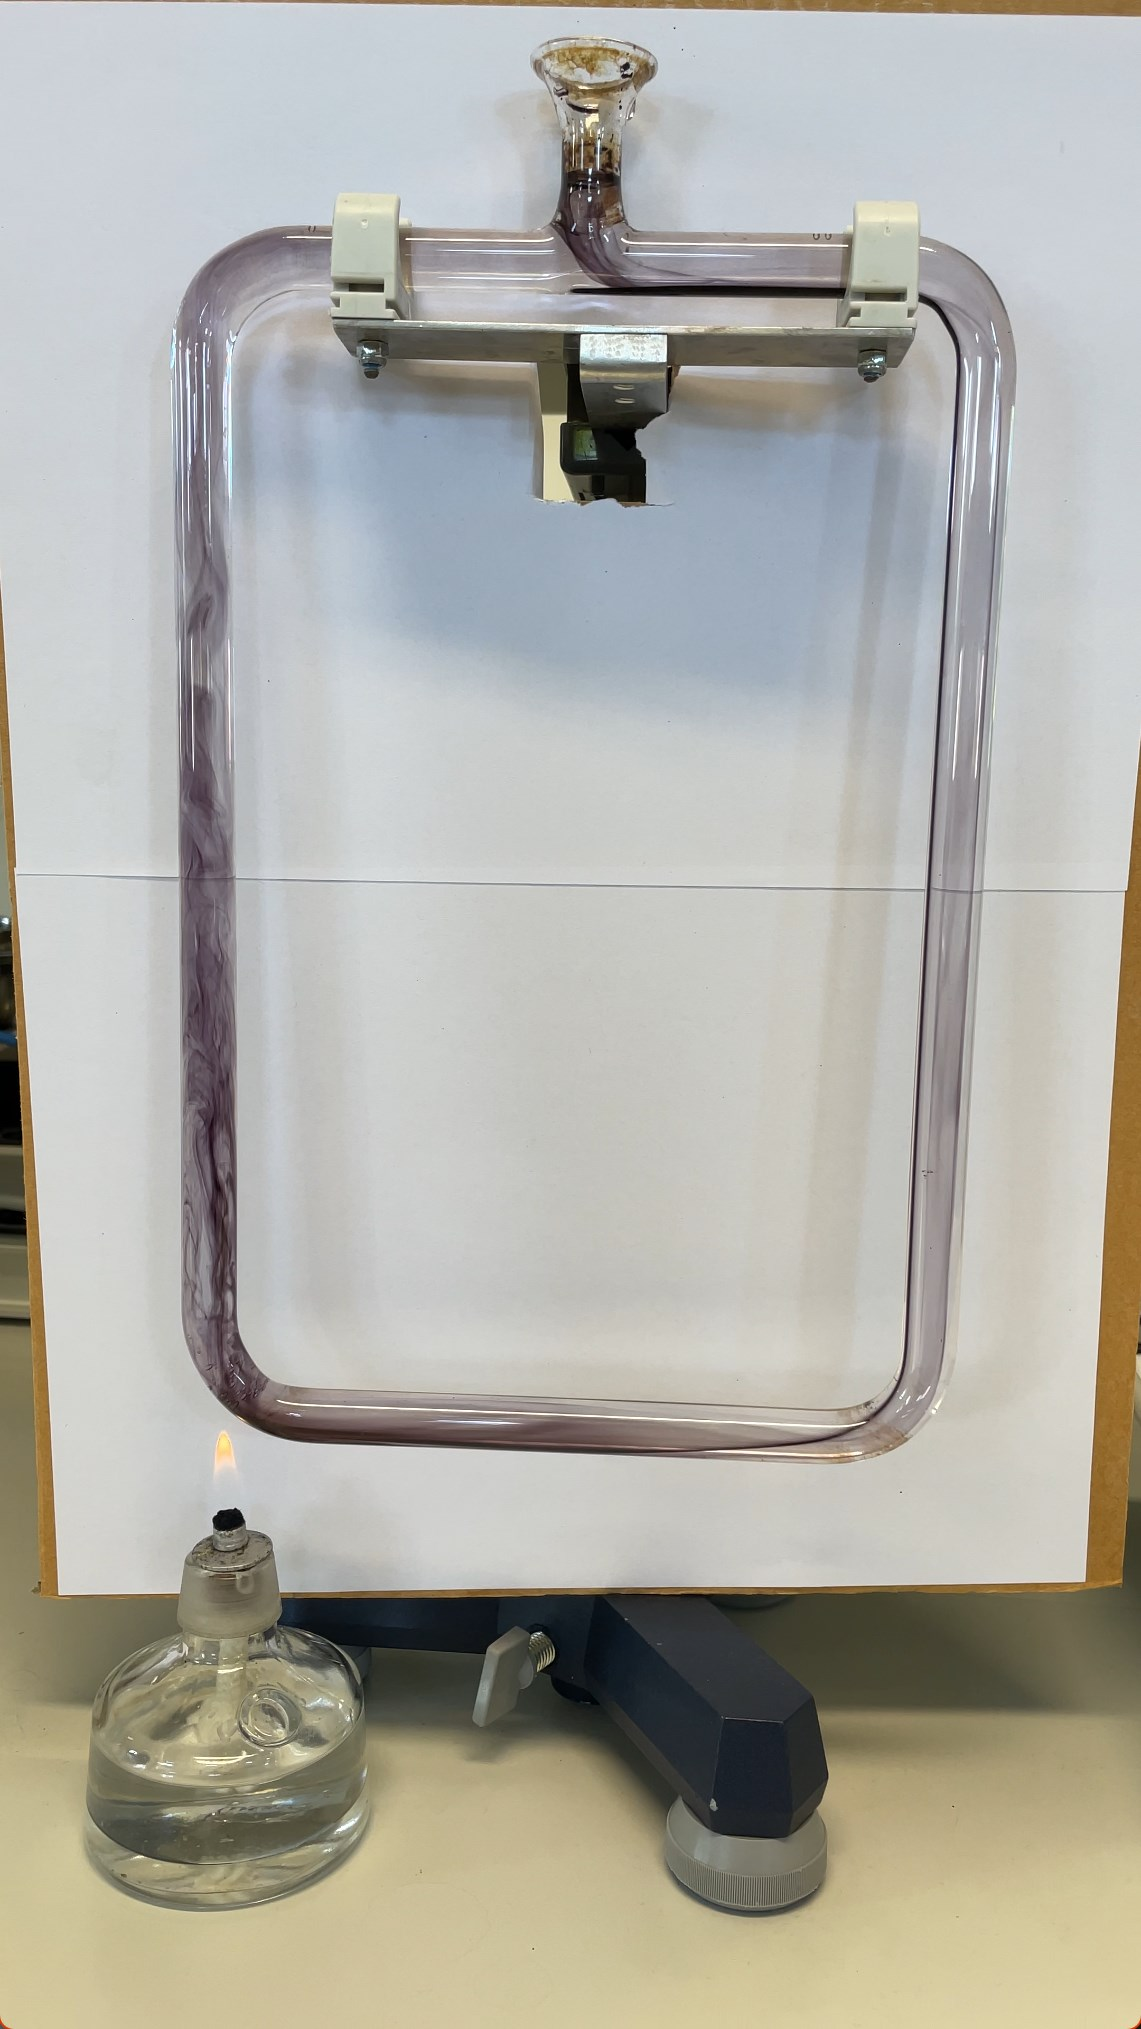
\includegraphics[width=4cm]{Abbildungen/4}
\caption{}
\label{d}
\end{subfigure}
\caption{}
\end{figure}

In Abbildung \ref{a} wird die Druckertinte in den Wasserkreislauf gegeben.
Durch den Spiritusbrennner hat das Wasser unterschiedliche Temperatur/Dichte.
Wie in Abbildung \ref{b} zu sehen fängt das Wasser dadurch an zu zirkulieren.
Das Wasser steigt an der Stelle des Spiritusbrenner auf, da dort seine Dichte niedriger ist (höhere Temperatur, siehe Abb. \ref{c}).
In der letzten Abbildung \ref{d} kann man sehen, dass das Wasser einmal im Kreis zirkuliert ist.

\newpage
\section{Wertung/Fazit}
Die gemessenen Werte liegen mit Toleranz in einem guten Bereich.
Die Ausgleichsfunktion die Excel berechnet hat liegt nah an unseren Messpunkten.
Auch die ausgerechneten Temperaturen zu den Widerständen liegen nah an unserer Messwertkurve.
Beim zweiten Versuch konnte man außerdem gut die Konvektion beobachten.
Insgesamt sind die Versuchsergebnisse zufriedenstellend.

\newpage
\section{Anhang}
\label{sec:Anhang}

\begin{table}[H]
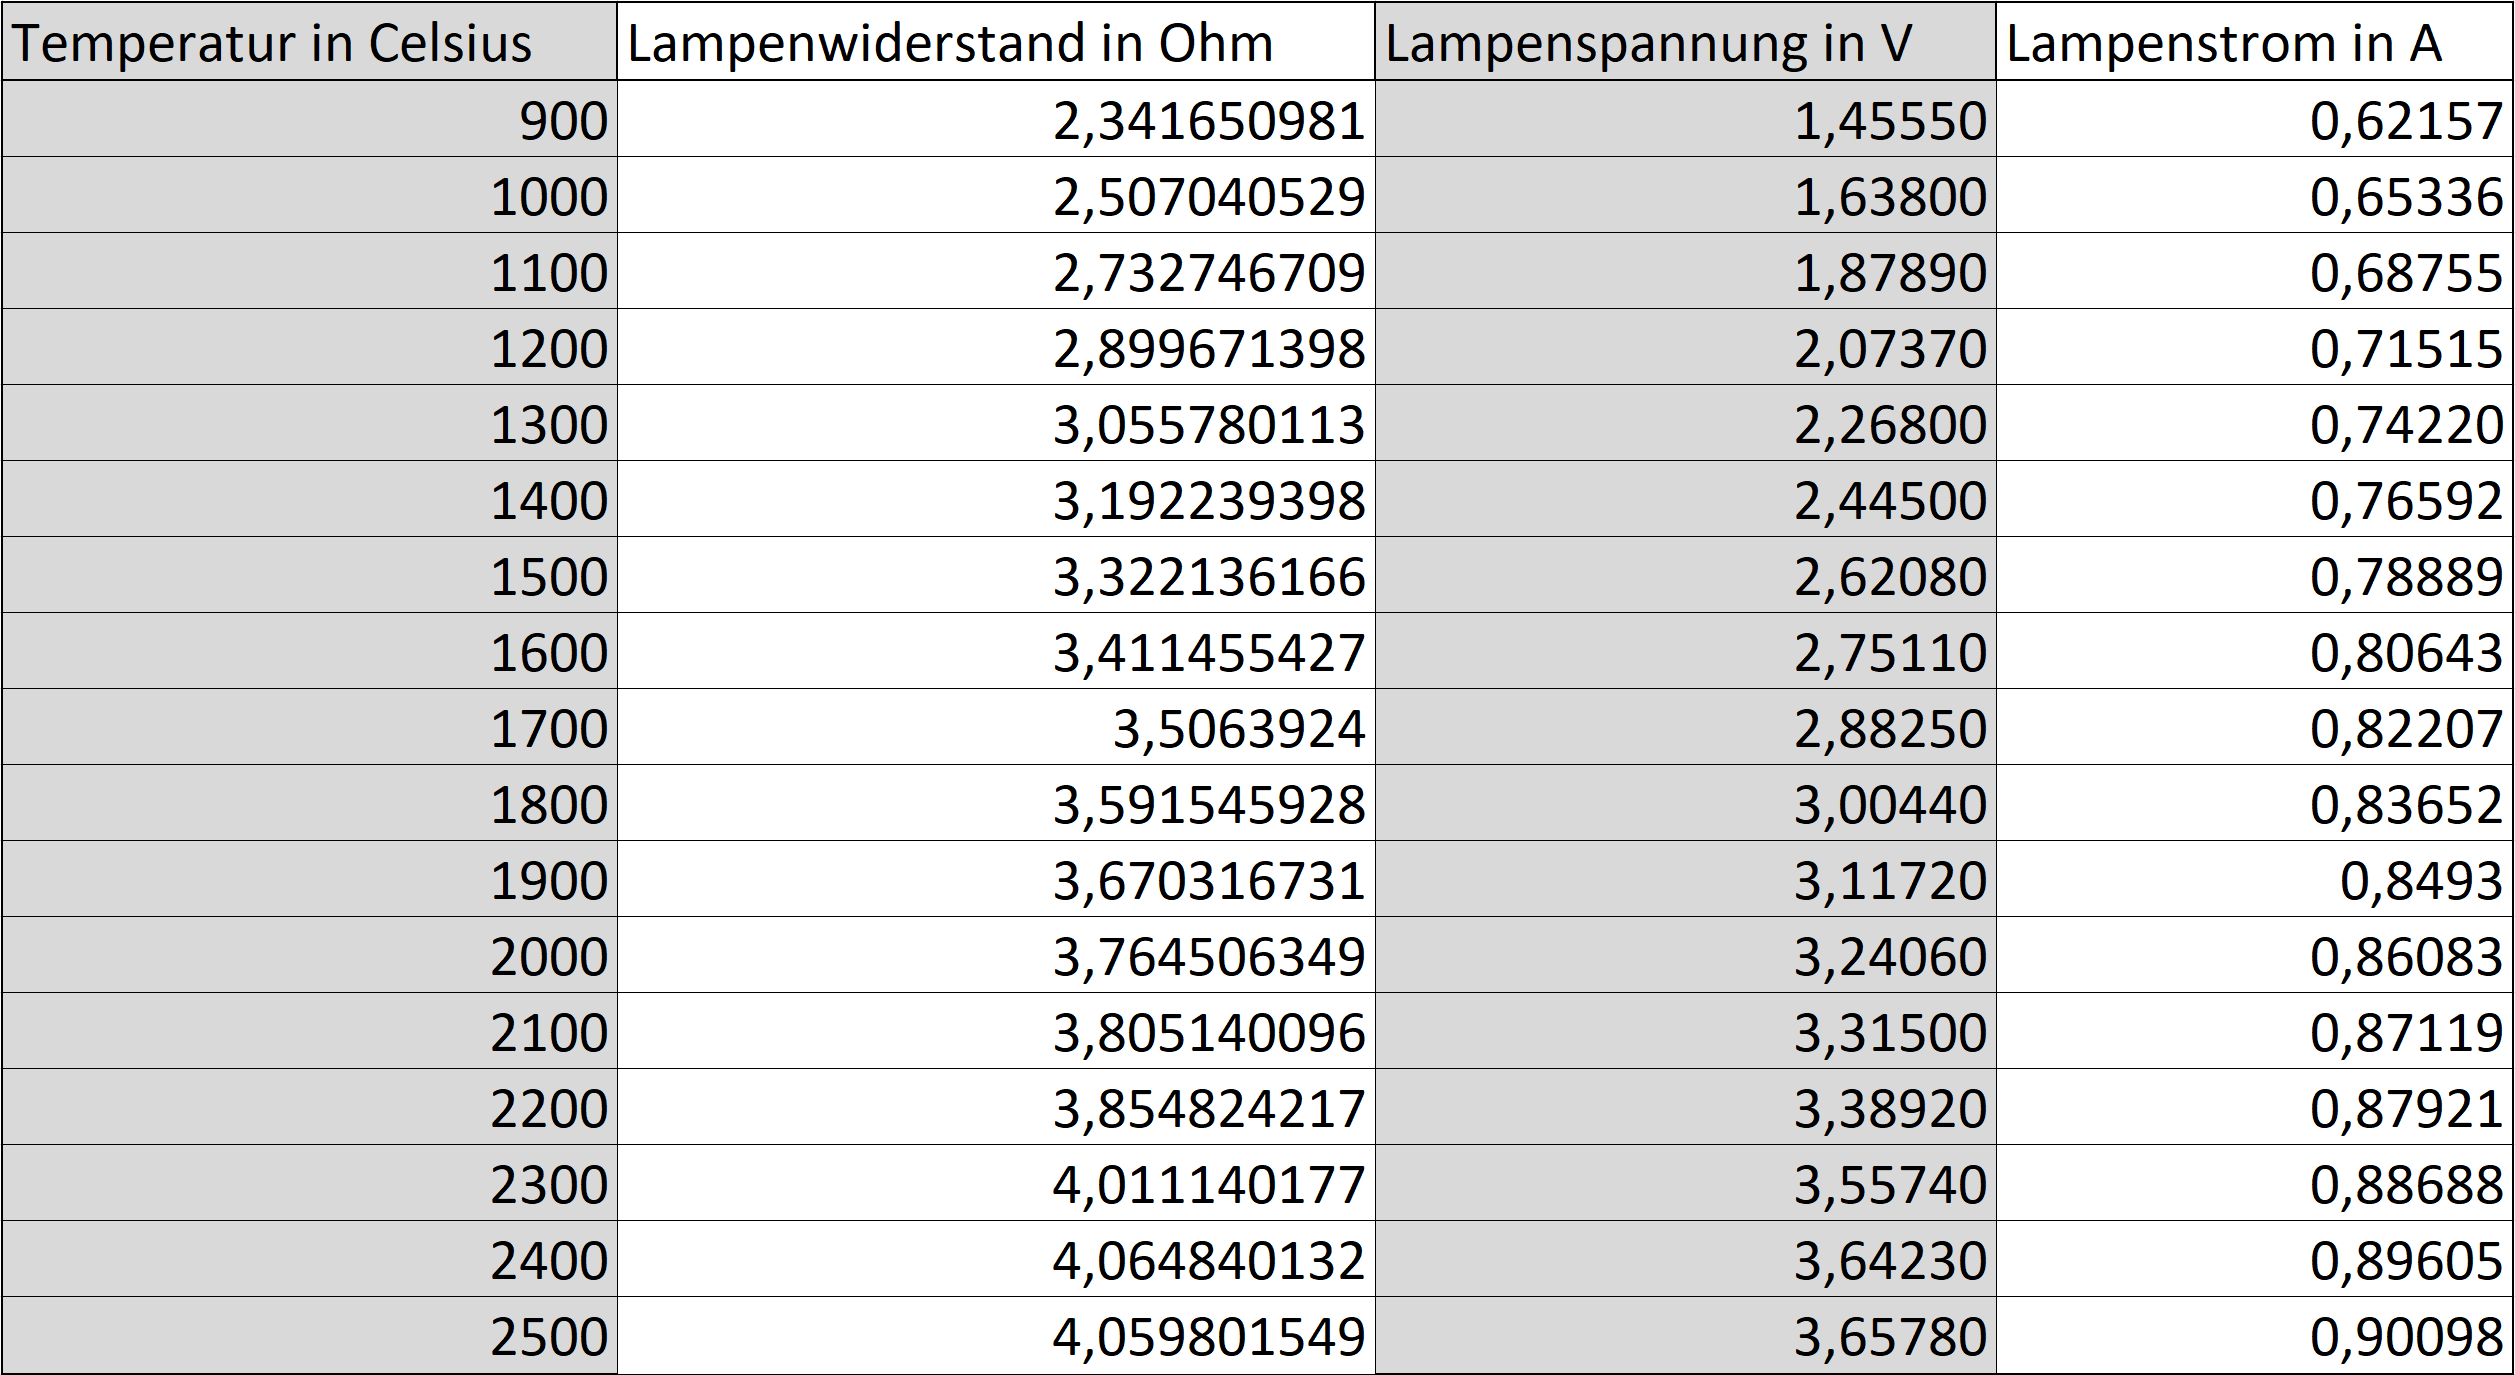
\includegraphics[width=12cm]{Abbildungen/Messwerte}
\centering
\caption{Messwerte}
\centering
\label{tab:Messwerte}
\end{table}

\begin{figure}[H]
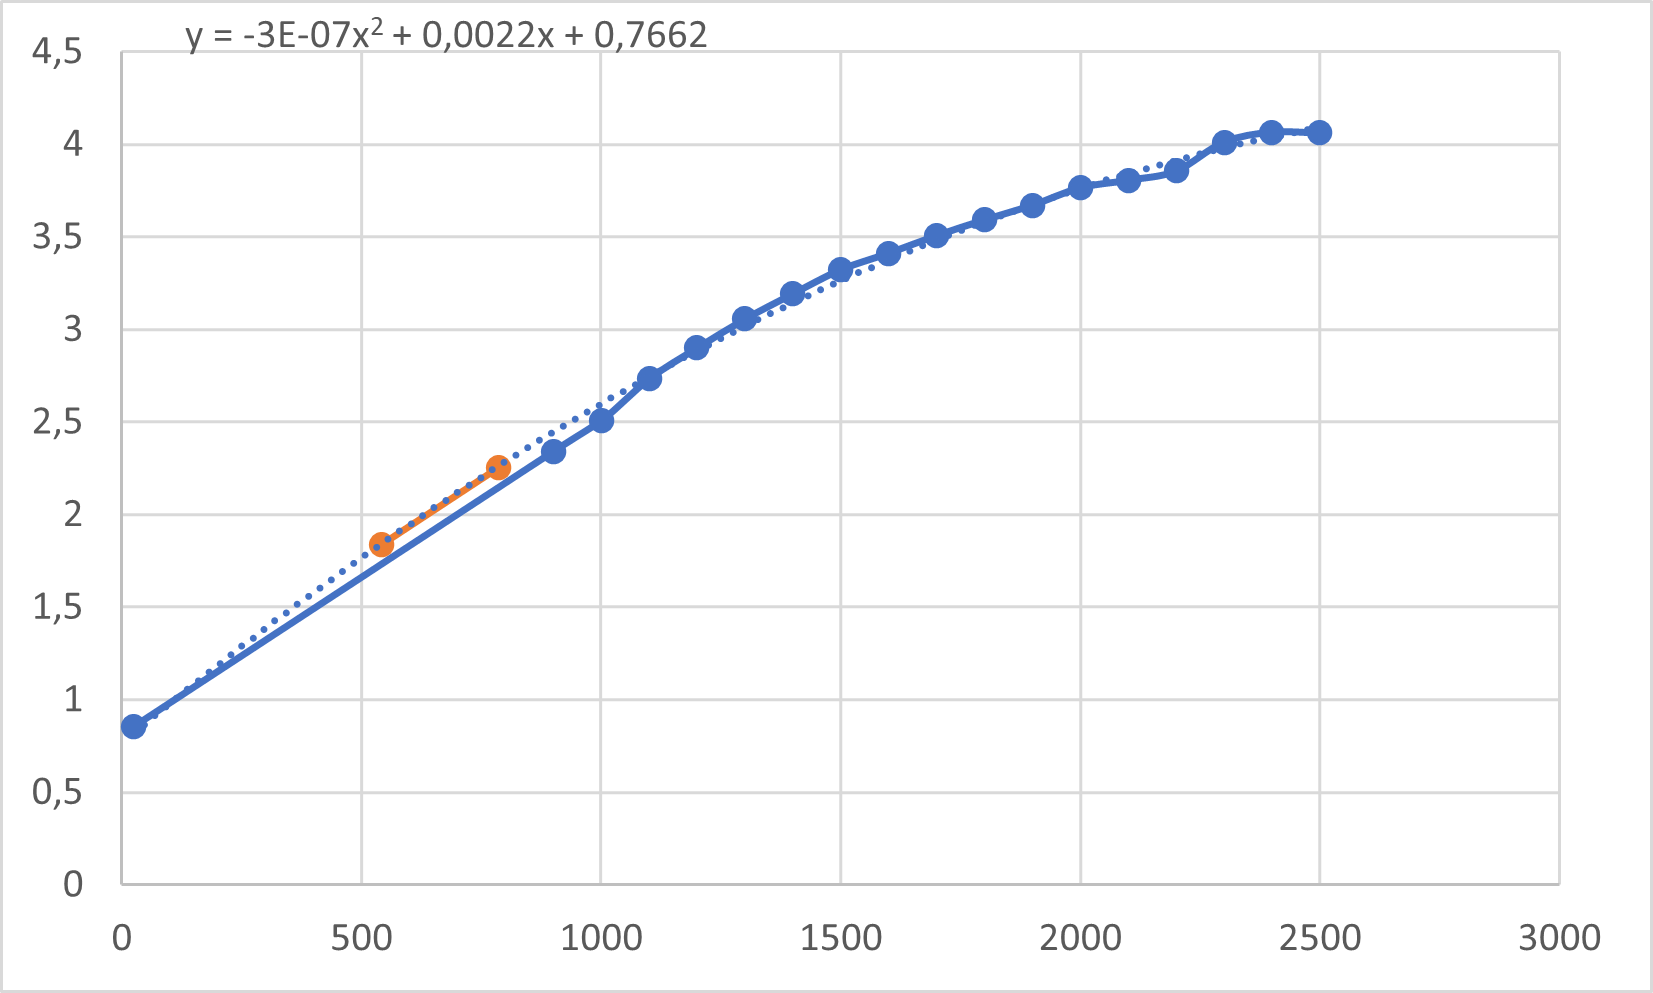
\includegraphics[width=12cm]{Abbildungen/Diagramm}
\centering
\caption{Diagramm Messwerte}
\centering
\label{fig:Diagramm}
\end{figure}

\begin{figure}[H]
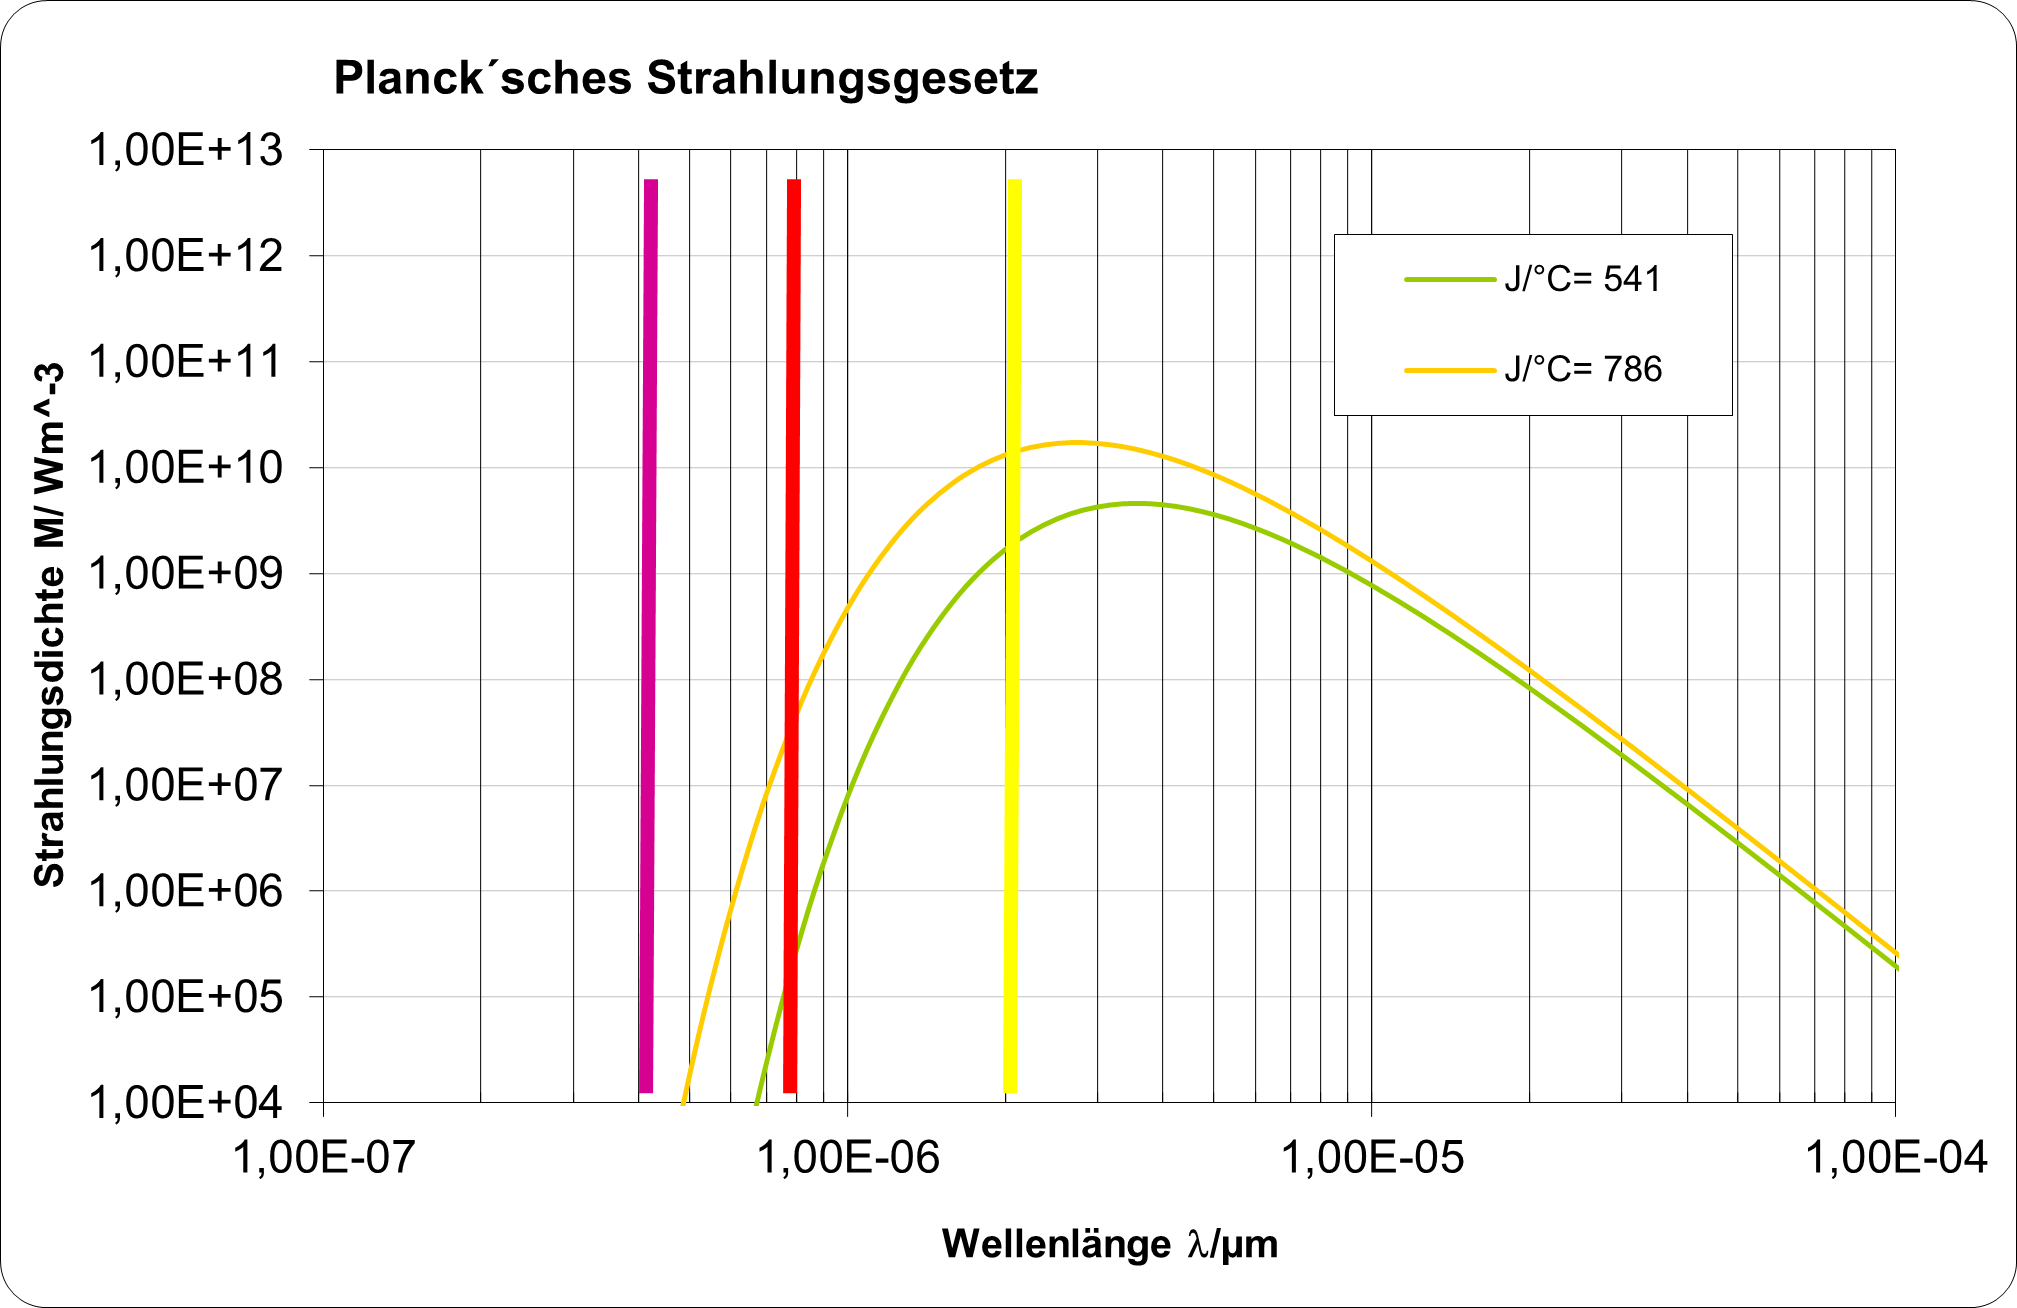
\includegraphics[width=12cm]{Abbildungen/Planck}
\centering
\caption{Planck Strahlengesetz Diagramm}
\centering
\end{figure}

\begin{figure}[H]
\includegraphics[width=12cm]{Abbildungen/Infrarotstrahler}
\centering
\caption{Infrarotstrahler}
\centering
\label{fig:IR}
\end{figure}

\newpage
\bibliography{literatur}

\label{LastPage}
\end{document}
%%% Local Variables:
%%% mode: latex
%%% TeX-master: t
%%% End:
